\documentclass{beamer}
\usetheme{tokitex}

\usepackage{tikz}
\usepackage{graphics}
\usepackage{multirow}
\usepackage{tabto}
\usepackage{xspace}
\usepackage{amsmath}

\usepackage{tikz}
\usepackage{clrscode3e}

\usepackage[english,bahasa]{babel}
\newtranslation[to=bahasa]{Section}{Bagian}
\newtranslation[to=bahasa]{Subsection}{Subbagian}

\usepackage{listings, lstautogobble}
\usepackage{color}

\definecolor{dkgreen}{rgb}{0,0.6,0}
\definecolor{gray}{rgb}{0.5,0.5,0.5}
\definecolor{mauve}{rgb}{0.58,0,0.82}

\lstset{frame=tb,
  language=pascal,
  aboveskip=1mm,
  belowskip=1mm,
  showstringspaces=false,
  columns=fullflexible,
  keepspaces=true,
  basicstyle={\small\ttfamily},
  numbers=none,
  numberstyle=\tiny\color{gray},
  keywordstyle=\color{blue},
  commentstyle=\color{dkgreen},
  stringstyle=\color{mauve},
  breaklines=true,
  breakatwhitespace=true,
  autogobble=true
}

\usepackage{caption}
\captionsetup[figure]{labelformat=empty}

\newcommand{\progTerm}[1]{\textbf{#1}}
\newcommand{\foreignTerm}[1]{\textit{#1}}
\newcommand{\newTerm}[1]{\alert{\textbf{#1}}}
\newcommand{\emp}[1]{\alert{#1}}
\newcommand{\statement}[1]{"#1"}

% Getting tired of writing \foreignTerm all the time
\newcommand{\farray}{\foreignTerm{array}\xspace}
\newcommand{\fArray}{\foreignTerm{Array}\xspace}
\newcommand{\foverhead}{\foreignTerm{overhead}\xspace}
\newcommand{\fOverhead}{\foreignTerm{Overhead}\xspace}
\newcommand{\fsubarray}{\foreignTerm{subarray}\xspace}
\newcommand{\fSubarray}{\foreignTerm{Subarray}\xspace}
\newcommand{\fbasecase}{\foreignTerm{base case}\xspace}
\newcommand{\fBasecase}{\foreignTerm{Base case}\xspace}
\newcommand{\ftopdown}{\foreignTerm{top down}\xspace}
\newcommand{\fTopdown}{\foreignTerm{Top down}\xspace}
\newcommand{\fbottomup}{\foreignTerm{bottom up}\xspace}
\newcommand{\fBottomup}{\foreignTerm{Bottom up}\xspace}
\newcommand{\fpruning}{\foreignTerm{pruning}\xspace}
\newcommand{\fPruning}{\foreignTerm{Pruning}\xspace}

\newcommand{\fgraph}{\foreignTerm{graph}\xspace}
\newcommand{\fGraph}{\foreignTerm{Graph}\xspace}
\newcommand{\fnode}{\foreignTerm{node}\xspace}
\newcommand{\fNode}{\foreignTerm{Node}\xspace}
\newcommand{\fedge}{\foreignTerm{edge}\xspace}
\newcommand{\fEdge}{\foreignTerm{Edge}\xspace}
\newcommand{\fdegree}{\foreignTerm{degree}\xspace}
\newcommand{\fDegree}{\foreignTerm{Degree}\xspace}
\newcommand{\fadjacencylist}{\foreignTerm{adjacency list}\xspace}
\newcommand{\fAdjacencylist}{\foreignTerm{Adjacency list}\xspace}
\newcommand{\fadjacencymatrix}{\foreignTerm{adjacency matrix}\xspace}
\newcommand{\fAdjacencymatrix}{\foreignTerm{Adjacency matrix}\xspace}
\newcommand{\fedgelist}{\foreignTerm{edge list}\xspace}
\newcommand{\fEdgelist}{\foreignTerm{Edge list}\xspace}
\newcommand{\flist}{\foreignTerm{list}\xspace}
\newcommand{\fList}{\foreignTerm{List}\xspace}
\newcommand{\fgraphtraversal}{\foreignTerm{graph traversal}\xspace}
\newcommand{\fGraphtraversal}{\foreignTerm{Graph traversal}\xspace}
\newcommand{\ftree}{\foreignTerm{tree}\xspace}
\newcommand{\fTree}{\foreignTerm{Tree}\xspace}

\newcommand{\fDivideAndConquer}{\foreignTerm{Divide and Conquer}\xspace}
\newcommand{\fMergeSort}{\foreignTerm{Merge Sort}\xspace}
\newcommand{\fQuickSort}{\foreignTerm{Quicksort}\xspace}
\newcommand{\fpivot}{\foreignTerm{pivot}\xspace}
\newcommand{\fPivot}{\foreignTerm{Pivot}\xspace}
\newcommand{\fBruteForce}{\foreignTerm{Brute Force}\xspace}
\newcommand{\fCompleteSearch}{\foreignTerm{Complete Search}\xspace}
\newcommand{\fExhaustiveSearch}{\foreignTerm{Exhaustive Search}\xspace}
\newcommand{\fBinarySearch}{\foreignTerm{Binary Search}\xspace}
\newcommand{\fGreedy}{\foreignTerm{Greedy}\xspace}
\newcommand{\fGreedyChoice}{\foreignTerm{Greedy Choice}\xspace}

\newcommand{\pheap}{\progTerm{heap}\xspace}
\newcommand{\pHeap}{\progTerm{Heap}\xspace}
\newcommand{\pBinaryHeap}{\progTerm{Binary Heap}\xspace}
\newcommand{\pbinaryHeap}{\progTerm{binary heap}\xspace}

\title{Struktur Data Non Linear: \newline Disjoint Set}
\author{Tim Olimpiade Komputer Indonesia}
\date{}

\begin{document}

\begin{frame}
\titlepage
\end{frame}

\begin{frame}
\frametitle{Pendahuluan}
Melalui dokumen ini, kalian akan:
\begin{itemize}
  \item Mengenal dan mengimplementasikan struktur data \pdjs.
  \item Mengetahui mengapa diperlukan \pdjs.
\end{itemize}
\end{frame}

\begin{frame}
\frametitle{Motivasi}
Terdapat $N$ orang di suatu ruangan, dinomori dari $1$ sampai dengan $N$. Secara bertahap, mereka membentuk suatu kelompok.\newline

Anda diberikan sejumlah operasi. Setiap operasi dapat berbentuk salah satu dari:
\begin{itemize}
  \item join($a$, $b$), artinya kelompok orang ke-$a$ dan kelompok orang ke-$b$ bergabung.
  \item check($a$, $b$), artinya periksa apakah orang ke-$a$ dan orang ke-$b$ sedang berada di kelompok yang sama.
\end{itemize}
\end{frame}

\begin{frame}
\frametitle{Contoh Perilaku}
Dengan $N=5$, Berikut contoh operasinya dan perilaku yang diharapkan:
\begin{itemize}
  \item Pada kondisi awal, setiap orang dapat dianggap membentuk kelompok sendiri $[1], [2], [3], [4], [5]$.
  \item join($1$, $4$), kini kelompok yang ada adalah $[1, 4], [2], [3], [5]$.
  \item check($1$, $2$): laporkan bahwa $1$ dan $2$ berada di kelompok berbeda.
  \item join($1$, $2$), kini kelompok yang ada adalah $[1, 2, 4], [3], [5]$.
  \item ...
\end{itemize}
\end{frame}

\begin{frame}
\frametitle{Contoh Perilaku (lanj.)}
\begin{itemize}
  \item ...
  \item check($1$, $2$): laporkan bahwa $1$ dan $2$ berada di kelompok yang sama.
  \item join($3$, $5$), kini kelompok yang ada adalah $[1, 2, 4], [3, 5]$.
  \item join($2$, $3$), kini kelompok yang ada adalah $[1, 2, 3, 4, 5]$.
  \item check($1$, $5$): laporkan bahwa $1$ dan $5$ berada di kelompok yang sama.
\end{itemize}
\end{frame}

\begin{frame}
\frametitle{Solusi Sederhana}
\begin{itemize}
  \item Dengan konsep \fgraph, representasikan setiap orang sebagai \fnode.
  \item Setiap operasi join dapat dianggap dengan penambahan \fedge.
  \item Untuk operasi check, diperlukan \fgraphtraversal untuk memeriksa apakah kedua \fnode terhubung.
  \item Representasi graf yang paling efisien untuk keperluan ini adalah \fadjacencylist.
\end{itemize}
\end{frame}

\begin{frame}
\frametitle{Analisis Solusi Sederhana}
\begin{table}[ht]
  \begin{tabular}{|l|c|}
    \hline Operasi  & Solusi Sederhana \\
    \hline  join($a$, $b$) & $O(1)$  \\
    \hline  check($a$, $b$) & $O(N)$ s/d $O(N^2)$\\
    \hline
  \end{tabular}
\end{table}  
Kompleksitas check mencapai $O(N^2)$ apabila \fgraphtraversal dilakukan secara naif dan seluruh kemungkinan \fedge dilalui.
\end{frame}

\begin{frame}
\frametitle{Masalah Solusi Sederhana}
\begin{itemize}
  \item Solusi sederhana ini jelas tidak efisien ketika banyak dilakukan operasi check($a$, $b$).
  \item Kita akan mempelajari bagaimana \pdjs mengatasi masalah ini secara efisien.
\end{itemize}
\end{frame}

\begin{frame}
\frametitle{Disjoint Set}
\begin{itemize}
  \item \pDjs merupakan struktur data yang efisien untuk mengelompokkan elemen-elemen secara bertahap.
  \item Operasi yang didukung adalah:
  \begin{itemize}
    \item \progTerm{Join}, yaitu menggabungkan kelompok dari sepasang elemen.
    \item \progTerm{Check}, yaitu memeriksa apakah sepasang elemen berada di kelompok yang sama.
  \end{itemize}
\end{itemize}
\end{frame}

\begin{frame}
\frametitle{Ide Dasar}
\begin{itemize}
  \item Untuk setiap kelompok yang ada, pilih suatu elemen sebagai "perwakilan kelompok".
  \item Setiap elemen perlu mengetahui siapa perwakilan kelompoknya.
  \item Untuk memeriksa apakah dua elemen berada pada kelompok yang sama, periksa apakah \textbf{perwakilan kelompok mereka sama}.
  \item Untuk menggabungkan kelompok dari dua elemen, \textbf{salah satu perwakilan kelompok elemen perlu diwakilkan oleh perwakilan kelompok elemen lainnya}.
\end{itemize}
\end{frame}

\begin{frame}
\frametitle{Cara Kerja Disjoint Set}
\begin{itemize}
  \item Setiap elemen perlu menyimpan \foreignTerm{pointer} ke elemen yang merupakan perwakilannya.
  \item \foreignTerm{Pointer} yang ditunjuk oleh suatu perwakilan kelompok adalah dirinya sendiri.
\end{itemize}
\begin{figure}
  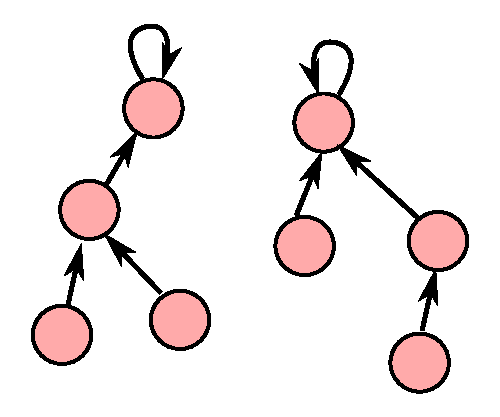
\includegraphics[width=4cm]{asset/djs.pdf}
\end{figure}
\end{frame}

\begin{frame}
\frametitle{Cara Kerja Disjoint Set (lanj.)}
\begin{itemize}
  \item Karena pada awalnya setiap elemen membentuk kelompoknya sendiri, maka awalnya setiap \foreignTerm{pointer} ini menunjuk pada dirinya sendiri.
  \item Untuk mempermudah, mari kita sebut \foreignTerm{pointer} ini sebagai \textbf{parent}.
\end{itemize}
\begin{figure}
  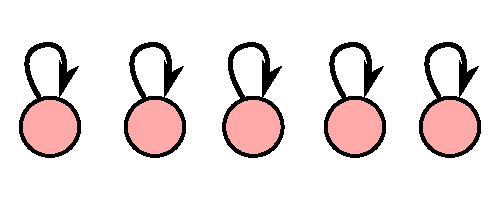
\includegraphics[width=5cm]{asset/djs-init.pdf}
\end{figure}
\end{frame}

\begin{frame}
\frametitle{Inisialisasi Disjoint Set}
Berikut prosedur inisialisasi \pdjs untuk $N$ elemen. \newline

Asumsikan \farray $par$ menyimpan indeks elemen yang ditunjuk sebagai \foreignTerm{parent} dari suatu elemen.
\begin{codebox}
\Procname{$\proc{initialize}()$}
\li \For $i \gets 0$ \To $N-1$ \Comment Indeks elemen dimulai dari 0 (zero based)
\li \Do   $par[i] = i$ 
    \End
\end{codebox}

Cukup sederhana, yaitu setiap elemen menunjuk ke dirinya sendiri.
\end{frame}

\begin{frame}
\frametitle{Operasi Join}
\begin{itemize}
  \item Ketika kelompok dua elemen perlu digabungkan, ubah \foreignTerm{parent} dari salah satu perwakilan kelompok ke kelompok lainnya.
\end{itemize}
\begin{figure}
  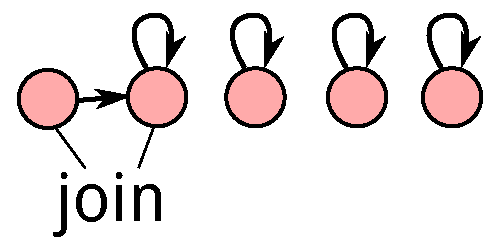
\includegraphics[width=5cm]{asset/djs-join-1.pdf}
\end{figure}
\end{frame}

\begin{frame}
\frametitle{Operasi Join (lanj.)}
\begin{itemize}
  \item Perhatikan bahwa yang perlu diubah adalah \foreignTerm{parent} dari perwakilan kelompok suatu elemen, bukan elemen itu sendiri.
\end{itemize}
\begin{figure}
  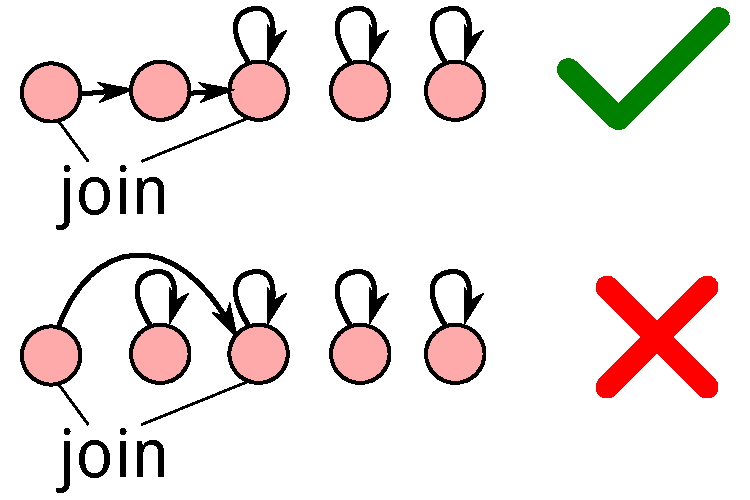
\includegraphics[width=7cm]{asset/djs-join-2.pdf}
\end{figure}
\end{frame}

\begin{frame}
\frametitle{Operasi Join (implementasi)}
Secara sederhana, operasi join dapat dituliskan dalam prosedur:

\begin{codebox}
\Procname{$\proc{join}(a, b)$}
\li $repA = \proc{findRepresentative}(a)$
\li $repB = \proc{findRepresentative}(b)$
\li $par[repA] = repB$
\end{codebox}

Fungsi $\proc{findRepresentative}(x)$ mengembalikan elemen perwakilan dari kelompok tempat elemen $x$ berada.
\end{frame}

\begin{frame}
\frametitle{Operasi Join (implementasi findRepresentative)}
Fungsi $\proc{findRepresentative}(x)$ dapat diimplementasikan secara rekursif, yaitu sampai ditemukan elemen yang memiliki \foreignTerm{parent} berupa dirinya sendiri.

\begin{codebox}
\Procname{$\proc{findRepresentative}(x)$}
\li \If $par[x] == x$ \Then
\li   \Return $x$
\li \Else
\li   \Return $\proc{findRepresentative}(par[x])$
    \End
\end{codebox}
\end{frame}

\begin{frame}
\frametitle{Kekurangan findRepresentative}
\begin{itemize}
  \item Fungsi $\proc{findRepresentative}$ memiliki kompleksitas sebesar $O(L)$, dengan $L$ adalah panjangnya jalur dari elemen $x$ sampai elemen perwakilan kelompoknya.
  \item Ketika $L$ mendekati $N$, fungsi ini tidak efisien bila dipanggil berkali-kali.
\end{itemize}
\begin{figure}
  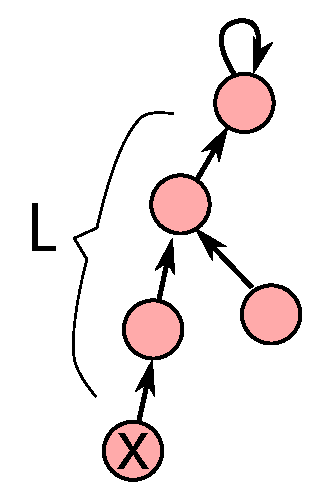
\includegraphics[width=3cm]{asset/chain-long.pdf}
\end{figure}
\end{frame}

\begin{frame}
\frametitle{Memperbaiki findRepresentative}
\begin{itemize}
  \item Kita dapat menerapkan teknik \textbf{"path compression"}, yaitu mengubah nilai \foreignTerm{parent} dari setiap elemen yang dilalui \textbf{langsung} ke elemen perwakilan kelompok.
  \item Hal ini menjamin untuk pemanggilan $\proc{findRepresentative}$ berikutnya pada elemen yang bersangkutan bekerja secara lebih efisien.
\end{itemize}
\begin{figure}
  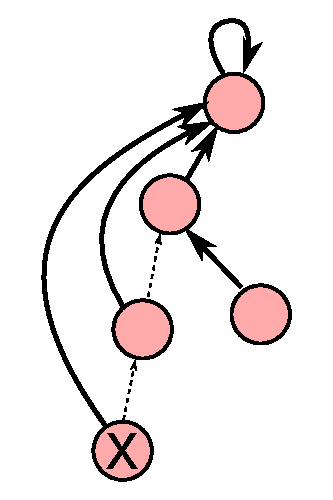
\includegraphics[width=3cm]{asset/chain-compressed.pdf}
\end{figure}
\end{frame}

\begin{frame}
\frametitle{Implementasi Path Compression}
Tambahkan pencatatan elemen perwakilan kelompok untuk setiap elemen yang dilalui.
\begin{codebox}
\Procname{$\proc{findRepresentative}(x)$}
\li \If $par[x] == x$ \Then
\li   \Return $x$
\li \Else
\li   \Comment Catat elemen representatifnya
\li   $par[x] = \proc{findRepresentative}(par[x])$ 
\li   \Return $par[x]$
    \End
\end{codebox}
\end{frame}

\begin{frame}
\frametitle{Analisis Kompleksitas findRepresentative}
\begin{itemize}
  \item Untuk \pdjs dengan $N$ elemen, paling banyak terdapat $N$ \foreignTerm{parent} yang dikenakan \foreignTerm{path compression}.
  \item Apabila seluruh \foreignTerm{parent} elemen sudah dikenakan \foreignTerm{path compression}, maka setiap elemen langsung menunjuk ke elemen perwakilan kelompoknya.
  \item Artinya, kini fungsi $\proc{findRepresentative}$ bekerja dalam $O(1)$.
\end{itemize}
\begin{figure}
  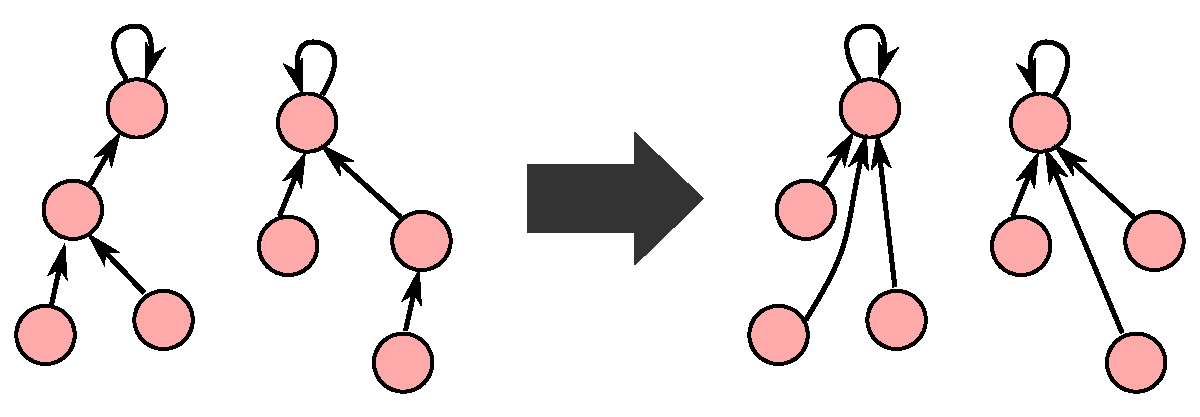
\includegraphics[width=10cm]{asset/djs-flat.pdf}
\end{figure}
\end{frame}

\begin{frame}
\frametitle{Analisis Kompleksitas findRepresentative (lanj.)}
\begin{itemize}
  \item Kompleksitas satu kali pemanggilan $\proc{findRepresentative}$ tidak dapat didefinisikan secara pasti.
  \item Yang pasti adalah, \textbf{kompleksitas total} untuk pemanggilan $\proc{findRepresentative}$ secara \textbf{berkali-kali} tidak akan lebih dari $O(N)$; sebab lebih dari itu dipastikan seluruh \foreignTerm{parent} sudah terkompresi secara merata.
  \item Setelah seluruh \foreignTerm{parent} terkompresi secara merata, kompleksitasnya adalah $O(1)$.
\end{itemize}
\end{frame}

\begin{frame}
\frametitle{Analisis Kompleksitas Join}
\begin{itemize}
  \item Kembali ke operasi join, kompleksitasnya bergantung pada $\proc{findRepresentative}$.
  \item Dapat dikatakan kompleksitas operasi join sama dengan kompleksitas $\proc{findRepresentative}$.
\end{itemize}
\end{frame}

\begin{frame}
\frametitle{Operasi Check}
\begin{itemize}
  \item Untuk operasi \foreignTerm{check}, cukup periksa apakah elemen perwakilan kelompok kedua elemen sama.
  \item Lagi-lagi, kompleksitas operasi \foreignTerm{check} sama dengan sama dengan kompleksitas $\proc{findRepresentative}$.
\end{itemize}
\begin{codebox}
\Procname{$\proc{check}(a, b)$}
\li   \Return $\proc{findRepresentative}(a) == \proc{findRepresentative}(b)$
\end{codebox}
\end{frame}

\begin{frame}
\frametitle{Penutup}
\begin{itemize}
  \item \pDjs merupakan struktur data yang sederhana dan mudah diimplementasikan.
  \item Biasanya struktur data ini dipakai untuk membantu implementasi algoritma lainnya, seperti \progTerm{Minimum Spanning Tree Kruskal}.
  \item Setiap Anda mengingat operasi "gabung" dan "periksa", ingatlah \pdjs.
\end{itemize}
\end{frame}

\end{document}


